\section{设计方案}
\subsection{总体设计思路}

总体设计思路分为两部分,第一部分为AXI的总体设计思路,主要包含mips向外部ram和外设进行交互的设计,第二部分为mips的总体设计思路,包含mips的流水线的设计\cite{cqu硬件综合文档}。

\subsubsection{AXI总体设计思路}

总体设计思路图如图\ref{figure1},这里以datapath向RAM请求数据为例,介绍总体设计思路。

首先datapath要请求数据时,将数据分为instruct数据和data数据,分别由i\_sram\_to\_sram\_like和d\_sram\_to\_sram\_like转换为sram\_like标准,也就是将inst\_req和data\_req设为1,并且等到地址握手后改变状态机,等待数据握手,并且将流水线stall。

对于inst\_req,只需要转换为物理地址后传给I\_Cache请求数据,若I\_Cache命中,则直接返回数据,若缺失,就将inst\_req传给cpu\_axi\_interface请求外部ram中的数据。

对于data\_req,首先要经过mmu,判断是否经过cache,若不经过cache,则通过1x2bridge将请求转给confreg\_data,直接请求外部Confreg,否则类似inst\_req,经过D\_Cache,后续和I\_Cache一致。

当外部传回数据的时候,也就是i\_sram\_to\_sram\_like和d\_sram\_to\_sram\_like接收到地址握手后,更改状态机,并将stall解除,然后由datapath把数据读出来。

\begin{figure}[H]
    \centering
    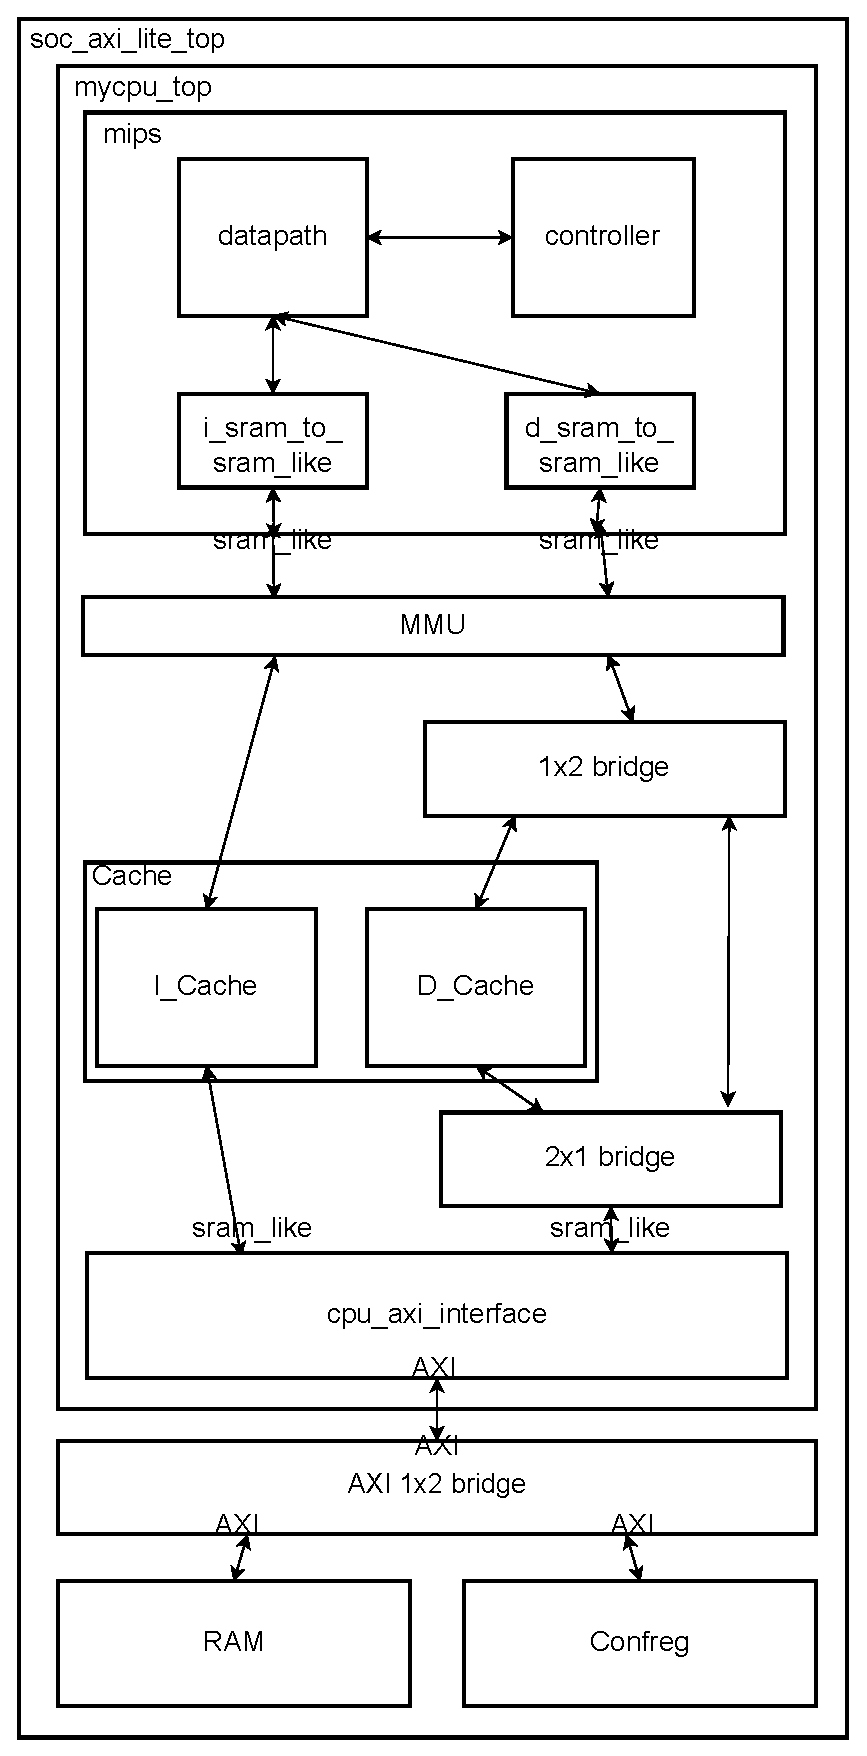
\includegraphics[width=0.6\textwidth]{image/totaldesign.eps}
    \caption{总体设计图}
    \label{figure1}
\end{figure}

\subsubsection{mips总体设计思路}

mips设计总体思路如图\ref{mips},总体上分为datapath,controller,i\_sram\_to\_sram\_like, d\_sram\_to\_sram\_like。

mips中,主要部分为datapath,datapath分为五级流水线,所有器件时钟同步,包含Fetch,Decode,Execute,Memory,Writeback五个阶段,以及冒险处理模块。Fetch阶段负责取指,指令地址由pcreg控制;Decode阶段将取到的指令交给controller进行译码,regfile负责读取相应寄存器的数据;Execute阶段根据controller译码的结果和regfile读取到的数据使用ALU进行计算,对于非除法指令,使用组合逻辑得到结果,对于除法,使用36周期除法器div得到结果,此时需要暂停流水线的全部阶段;Memory阶段负责memory数据,hilo数据,cp0数据的存储和读取,memwritedata负责写入数据的处理,主要处理的是sb和sh指令,memreaddata负责处理memory得到的数据,主要处理的是lb(u)和lh(u)指令,memlwexception负责处理读取指令的地址例外,exception模块将前面得到的异常汇总,通过组合逻辑得出exception的类型传给cp0处理,并且确定Fetch阶段下一跳的地址;Writeback阶段,将相应数据写入到regfile中。

在controller中,maindec根据decode阶段传入的指令翻译出各个组件的控制型号,aludec根据decode阶段传入的指令翻译出alu的运算类型。

\begin{figure}
    \centering
    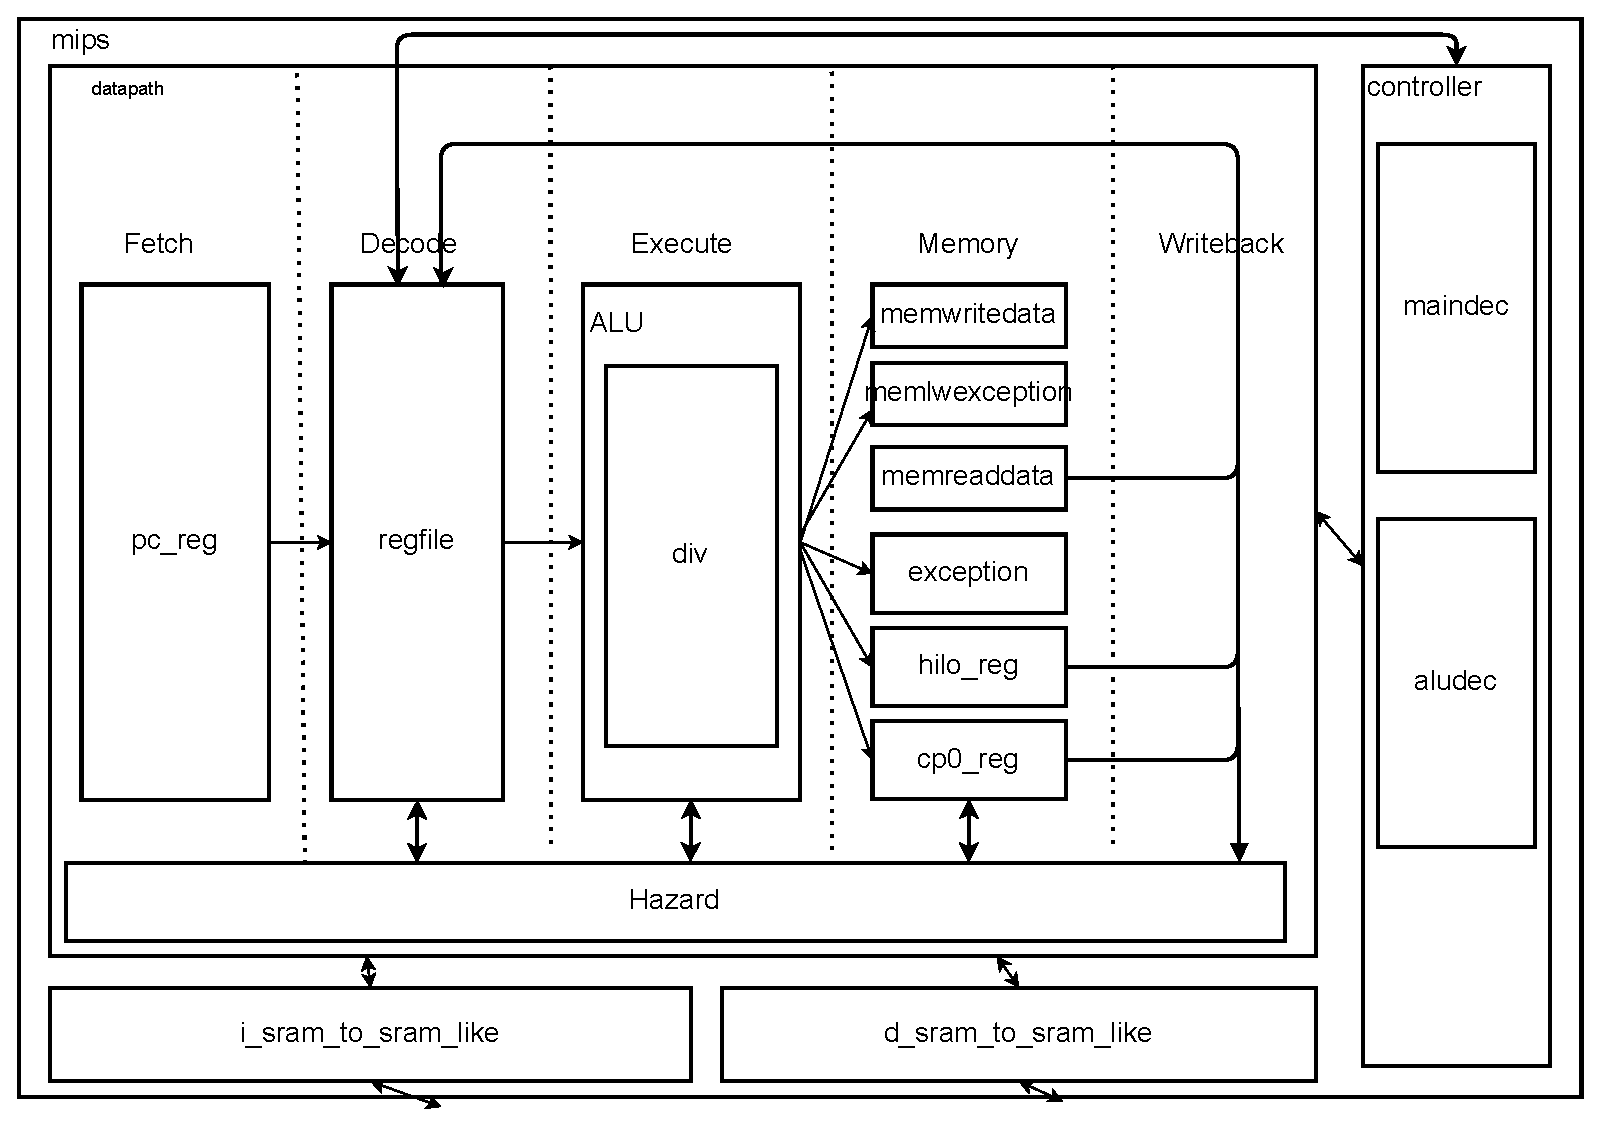
\includegraphics[width=\textwidth]{image/mips.eps}
    \caption{mips设计图}
    \label{mips}
\end{figure}


\subsection{写透d\_cache模块设计}

cache部分理解了ref\_code中的cache后直接使用了其中的写透cache,由于i\_cache只需要读,设计是d\_cache的子集,因此此处只对d\_cache进行说明。

其接口定义如下:

\begin{table}[H]
    \centering
    \begin{tabular}{ccccc}
        \hline
        信号名 & 方向 & 接口类型 & 位宽 & 说明 \\\hline
        clk & input & wire & 1 & 时钟 \\ 
        rst & input & wire & 1 & 复位信号 \\ 
        cpu\_data\_req & input & wire & 1 & 发送的请求 \\ 
        cpu\_data\_wr & input & wire & 1 & 是否是写请求 \\ 
        cpu\_data\_size & input & wire & 2 & 配合addr的最后两位决定有效字节 \\ 
        cpu\_data\_addr & input & wire & 32 & 写或读地址 \\ 
        cpu\_data\_wdata & input & wire & 32 & 写数据 \\ 
        cpu\_data\_rdata & output & wire & 32 & 读出来的数据 \\ 
        cpu\_data\_addr\_ok & output & wire & 1 & 地址握手 \\ 
        cpu\_data\_data\_ok & output & wire & 1 & 数据握手 \\ 
        cache\_data\_req & output & wire & 1 & 发送的请求 \\ 
        cache\_data\_wr & output & wire & 1 & 是否是写请求 \\ 
        cache\_data\_size & output & wire & 2 & 配合addr的最后两位决定有效字节 \\ 
        cache\_data\_addr & output & wire & 32 & 写或读地址 \\ 
        cache\_data\_wdata & output & wire & 32 & 写数据 \\ 
        cache\_data\_rdata & input & wire & 32 & 读出来的数据 \\ 
        cache\_data\_addr\_ok & input & wire & 1 & 地址握手 \\ 
        cache\_data\_data\_ok & input & wire & 1 & 数据握手 \\ 

        \hline
    \end{tabular}
\end{table}

这里需要注意的是cpu\_开头的代表cpu与cache之间的交互,cache\_开头的是cache与外部axi的交互。

cache中的状态机定义如下:
\begin{figure}[H]
    \centering
    \tikzset{every picture/.style={line width=0.75pt}} %set default line width to 0.75pt        

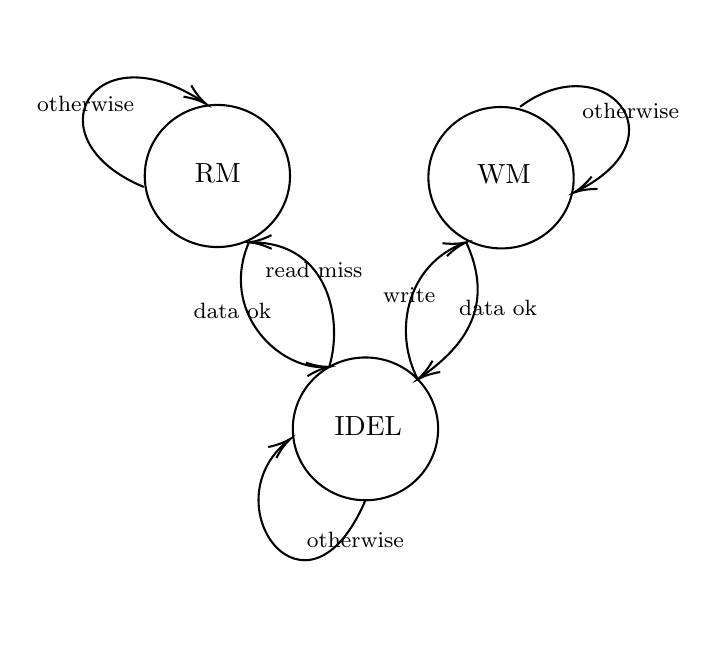
\begin{tikzpicture}[x=0.75pt,y=0.75pt,yscale=-1,xscale=1]
%uncomment if require: \path (0,375); %set diagram left start at 0, and has height of 375

%Shape: Ellipse [id:dp19171149818906597] 
\draw   (171.33,101.23) .. controls (171.33,82.33) and (187,67) .. (206.33,67) .. controls (225.66,67) and (241.33,82.33) .. (241.33,101.23) .. controls (241.33,120.14) and (225.66,135.47) .. (206.33,135.47) .. controls (187,135.47) and (171.33,120.14) .. (171.33,101.23) -- cycle ;
%Shape: Ellipse [id:dp4428011587585383] 
\draw   (308,102.07) .. controls (307.89,83.25) and (323.47,68) .. (342.8,68) .. controls (362.13,68) and (377.89,83.25) .. (378,102.07) .. controls (378.11,120.88) and (362.53,136.13) .. (343.2,136.13) .. controls (323.87,136.13) and (308.11,120.88) .. (308,102.07) -- cycle ;

%Shape: Ellipse [id:dp1811717312604948] 
\draw   (242.67,223.07) .. controls (242.67,204.07) and (258.34,188.67) .. (277.67,188.67) .. controls (297,188.67) and (312.67,204.07) .. (312.67,223.07) .. controls (312.67,242.07) and (297,257.47) .. (277.67,257.47) .. controls (258.34,257.47) and (242.67,242.07) .. (242.67,223.07) -- cycle ;

%Curve Lines [id:da1983440712749498] 
\draw    (260.2,193.2) .. controls (266.77,172.19) and (261.04,133.71) .. (223.28,133.2) ;
\draw [shift={(221.53,133.2)}, rotate = 359.03] [color={rgb, 255:red, 0; green, 0; blue, 0 }  ][line width=0.75]    (10.93,-3.29) .. controls (6.95,-1.4) and (3.31,-0.3) .. (0,0) .. controls (3.31,0.3) and (6.95,1.4) .. (10.93,3.29)   ;
%Curve Lines [id:da37604616095390786] 
\draw    (221.53,133.2) .. controls (207.23,166.35) and (235.39,194.43) .. (258.44,193.34) ;
\draw [shift={(260.2,193.2)}, rotate = 173.48] [color={rgb, 255:red, 0; green, 0; blue, 0 }  ][line width=0.75]    (10.93,-3.29) .. controls (6.95,-1.4) and (3.31,-0.3) .. (0,0) .. controls (3.31,0.3) and (6.95,1.4) .. (10.93,3.29)   ;
%Curve Lines [id:da7523161377824554] 
\draw    (302.87,199.2) .. controls (290.45,175.03) and (298.53,143.81) .. (324.58,133.79) ;
\draw [shift={(326.2,133.2)}, rotate = 161.15] [color={rgb, 255:red, 0; green, 0; blue, 0 }  ][line width=0.75]    (10.93,-3.29) .. controls (6.95,-1.4) and (3.31,-0.3) .. (0,0) .. controls (3.31,0.3) and (6.95,1.4) .. (10.93,3.29)   ;
%Curve Lines [id:da6823297551745142] 
\draw    (326.2,133.2) .. controls (341.72,166.83) and (321.49,186.03) .. (304.44,198.1) ;
\draw [shift={(302.87,199.2)}, rotate = 325.3] [color={rgb, 255:red, 0; green, 0; blue, 0 }  ][line width=0.75]    (10.93,-3.29) .. controls (6.95,-1.4) and (3.31,-0.3) .. (0,0) .. controls (3.31,0.3) and (6.95,1.4) .. (10.93,3.29)   ;
%Curve Lines [id:da12404472500434971] 
\draw    (170.87,106.53) .. controls (115.43,83.43) and (146.24,30.28) .. (199.25,65.44) ;
\draw [shift={(200.87,66.53)}, rotate = 214.66] [color={rgb, 255:red, 0; green, 0; blue, 0 }  ][line width=0.75]    (10.93,-3.29) .. controls (6.95,-1.4) and (3.31,-0.3) .. (0,0) .. controls (3.31,0.3) and (6.95,1.4) .. (10.93,3.29)   ;
%Curve Lines [id:da8562650717833464] 
\draw    (352.2,67.87) .. controls (391.8,38.17) and (432.05,82.3) .. (379.81,108.41) ;
\draw [shift={(378.2,109.2)}, rotate = 334.56] [color={rgb, 255:red, 0; green, 0; blue, 0 }  ][line width=0.75]    (10.93,-3.29) .. controls (6.95,-1.4) and (3.31,-0.3) .. (0,0) .. controls (3.31,0.3) and (6.95,1.4) .. (10.93,3.29)   ;
%Curve Lines [id:da24093253155107752] 
\draw    (277.67,257.47) .. controls (249.15,323.86) and (202.48,259.19) .. (240.36,228.78) ;
\draw [shift={(241.53,227.87)}, rotate = 143.13] [color={rgb, 255:red, 0; green, 0; blue, 0 }  ][line width=0.75]    (10.93,-3.29) .. controls (6.95,-1.4) and (3.31,-0.3) .. (0,0) .. controls (3.31,0.3) and (6.95,1.4) .. (10.93,3.29)   ;

% Text Node
\draw (329.94,94.42) node [anchor=north west][inner sep=0.75pt]   [align=left] {WM};
% Text Node
\draw (194,93.59) node [anchor=north west][inner sep=0.75pt]   [align=left] {RM};
% Text Node
\draw (261.33,215.43) node [anchor=north west][inner sep=0.75pt]   [align=left] {IDEL};
% Text Node
\draw (228,141) node [anchor=north west][inner sep=0.75pt]   [align=left] {{\footnotesize read miss}};
% Text Node
\draw (193.33,161) node [anchor=north west][inner sep=0.75pt]   [align=left] {{\footnotesize data ok}};
% Text Node
\draw (321.33,159.67) node [anchor=north west][inner sep=0.75pt]   [align=left] {{\footnotesize data ok}};
% Text Node
\draw (284.67,153.33) node [anchor=north west][inner sep=0.75pt]   [align=left] {{\footnotesize write}};
% Text Node
\draw (118,61.33) node [anchor=north west][inner sep=0.75pt]  [font=\normalsize] [align=left] {{\footnotesize otherwise}};
% Text Node
\draw (380.67,64.67) node [anchor=north west][inner sep=0.75pt]   [align=left] {{\footnotesize otherwise}};
% Text Node
\draw (248,271.33) node [anchor=north west][inner sep=0.75pt]   [align=left] {{\footnotesize otherwise}};


\end{tikzpicture}
\caption{dcache状态机}
\end{figure}

cache的组织方式(通路图)如下:
\begin{figure}[H]
    \centering
    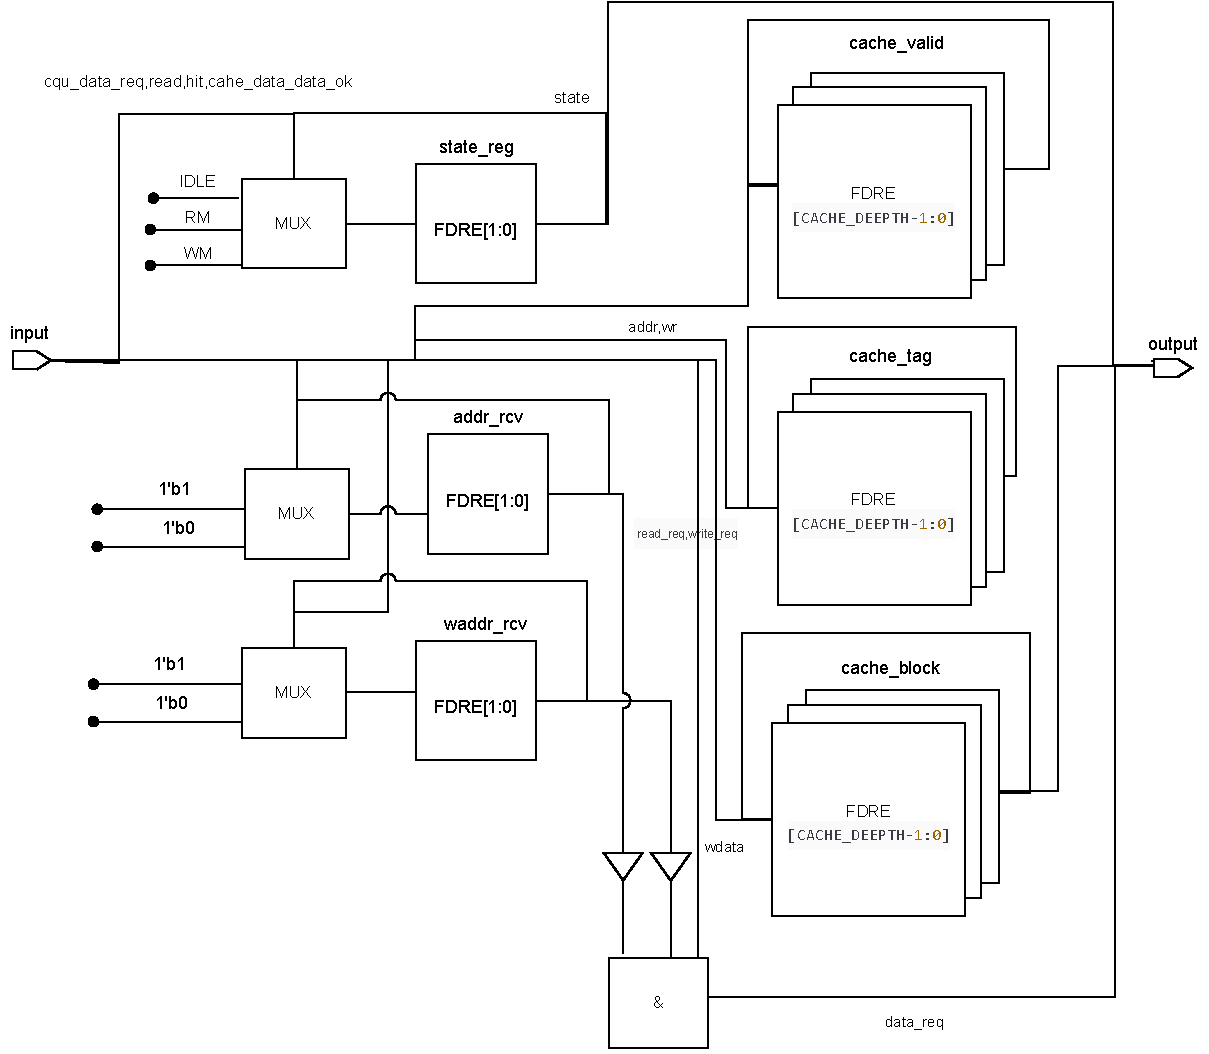
\includegraphics[width=0.9\textwidth]{image/dcachepath.pdf}
    \caption{dcache通路图}
\end{figure}


\subsection{sram\_to\_sram\_like模块设计}

该部分参考系统结构实验二的结构,其模块接口定义如下(X代表inst或者data):
\begin{table}[H]
    \centering
    \begin{tabular}{ccccc}
        \hline
        信号名 & 方向 & 接口类型 & 位宽 & 说明 \\\hline
        clk & input & wire & 1 & 时钟 \\ 
        rst & input & wire & 1 & 复位信号 \\ 
        X\_sram\_en & input & wire & 1 & ram使能 \\ 
        X\_sram\_addr & input & wire & 32 & 读ram的地址 \\ 
        X\_sram\_rdata & output & wire & 32 & ram读出来的数据 \\  
        X\_stall & output & wire & 1 & 操作ram时带来的stall \\  
        X\_req & output & wire & 1 & 发起的数据请求 \\ 
        X\_wr & output & wire & 1 & 是否是写请求 \\ 
        X\_size & output & wire & 2 & 配合addr的最后两位决定操作ram的有效字节 \\ 
        X\_addr & output & wire & 32 & 读或写的地址 \\ 
        X\_wdata & output & wire & 32 & 写入的值 \\ 
        X\_addr\_ok & input & wire & 1 & 地址握手信号 \\ 
        X\_data\_ok & input & wire & 1 & 数据握手信号 \\ 
        X\_rdata & input & wire & 32 & 读出的数据 \\ 
        all\_stall & input & wire & 1 & 是否正在全阶段stall \\ 

        \hline
    \end{tabular}
\end{table}

在模块中使用addr\_rcv来记录地址握手的状态,利用do\_finish来记录是否拿到了有效数据。模块内部判断地址握手和数据握手的状态机如下:
\begin{figure}[H]
\centering

\tikzset{every picture/.style={line width=0.75pt}} %set default line width to 0.75pt        

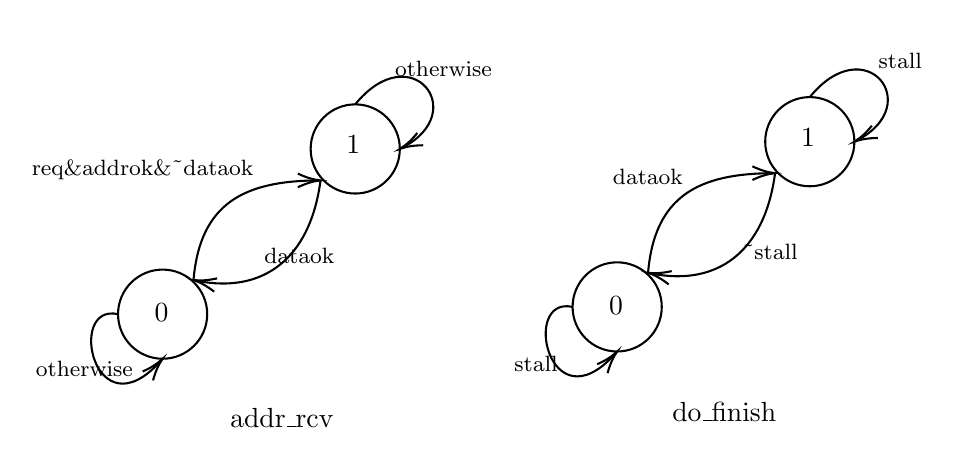
\begin{tikzpicture}[x=0.75pt,y=0.75pt,yscale=-1,xscale=1]
%uncomment if require: \path (0,310); %set diagram left start at 0, and has height of 310

%Shape: Circle [id:dp33032545980408967] 
\draw   (167.84,110.88) .. controls (167.84,99.02) and (177.46,89.4) .. (189.32,89.4) .. controls (201.18,89.4) and (210.8,99.02) .. (210.8,110.88) .. controls (210.8,122.74) and (201.18,132.36) .. (189.32,132.36) .. controls (177.46,132.36) and (167.84,122.74) .. (167.84,110.88) -- cycle ;
%Shape: Circle [id:dp4051114559339719] 
\draw   (75.04,190.48) .. controls (75.04,178.62) and (84.66,169) .. (96.52,169) .. controls (108.38,169) and (118,178.62) .. (118,190.48) .. controls (118,202.34) and (108.38,211.96) .. (96.52,211.96) .. controls (84.66,211.96) and (75.04,202.34) .. (75.04,190.48) -- cycle ;
%Curve Lines [id:da7708921388191468] 
\draw    (111.4,174.04) .. controls (114.55,136.61) and (136.33,126.35) .. (171.01,126.05) ;
\draw [shift={(172.6,126.04)}, rotate = 180] [color={rgb, 255:red, 0; green, 0; blue, 0 }  ][line width=0.75]    (10.93,-3.29) .. controls (6.95,-1.4) and (3.31,-0.3) .. (0,0) .. controls (3.31,0.3) and (6.95,1.4) .. (10.93,3.29)   ;
%Curve Lines [id:da8993376814012368] 
\draw    (172.6,126.04) .. controls (167.5,164.46) and (144.35,180.59) .. (113.31,174.44) ;
\draw [shift={(111.4,174.04)}, rotate = 12.68] [color={rgb, 255:red, 0; green, 0; blue, 0 }  ][line width=0.75]    (10.93,-3.29) .. controls (6.95,-1.4) and (3.31,-0.3) .. (0,0) .. controls (3.31,0.3) and (6.95,1.4) .. (10.93,3.29)   ;
%Curve Lines [id:da9519104737913102] 
\draw    (75.04,190.48) .. controls (50.05,184.9) and (63.52,248.74) .. (95.54,213.07) ;
\draw [shift={(96.52,211.96)}, rotate = 130.67] [color={rgb, 255:red, 0; green, 0; blue, 0 }  ][line width=0.75]    (10.93,-3.29) .. controls (6.95,-1.4) and (3.31,-0.3) .. (0,0) .. controls (3.31,0.3) and (6.95,1.4) .. (10.93,3.29)   ;
%Curve Lines [id:da2143048212569565] 
\draw    (189.32,89.4) .. controls (216.09,56.45) and (245.12,92.83) .. (212.34,110.1) ;
\draw [shift={(210.8,110.88)}, rotate = 334.31] [color={rgb, 255:red, 0; green, 0; blue, 0 }  ][line width=0.75]    (10.93,-3.29) .. controls (6.95,-1.4) and (3.31,-0.3) .. (0,0) .. controls (3.31,0.3) and (6.95,1.4) .. (10.93,3.29)   ;

%Shape: Circle [id:dp9355659130870222] 
\draw   (386.84,107.38) .. controls (386.84,95.52) and (396.46,85.9) .. (408.32,85.9) .. controls (420.18,85.9) and (429.8,95.52) .. (429.8,107.38) .. controls (429.8,119.24) and (420.18,128.86) .. (408.32,128.86) .. controls (396.46,128.86) and (386.84,119.24) .. (386.84,107.38) -- cycle ;
%Shape: Circle [id:dp38783632310043514] 
\draw   (294.04,186.98) .. controls (294.04,175.12) and (303.66,165.5) .. (315.52,165.5) .. controls (327.38,165.5) and (337,175.12) .. (337,186.98) .. controls (337,198.84) and (327.38,208.46) .. (315.52,208.46) .. controls (303.66,208.46) and (294.04,198.84) .. (294.04,186.98) -- cycle ;
%Curve Lines [id:da1889569445470416] 
\draw    (330.4,170.54) .. controls (333.55,133.11) and (355.33,122.85) .. (390.01,122.55) ;
\draw [shift={(391.6,122.54)}, rotate = 180] [color={rgb, 255:red, 0; green, 0; blue, 0 }  ][line width=0.75]    (10.93,-3.29) .. controls (6.95,-1.4) and (3.31,-0.3) .. (0,0) .. controls (3.31,0.3) and (6.95,1.4) .. (10.93,3.29)   ;
%Curve Lines [id:da2843375335727887] 
\draw    (391.6,122.54) .. controls (386.5,160.96) and (363.35,177.09) .. (332.31,170.94) ;
\draw [shift={(330.4,170.54)}, rotate = 12.68] [color={rgb, 255:red, 0; green, 0; blue, 0 }  ][line width=0.75]    (10.93,-3.29) .. controls (6.95,-1.4) and (3.31,-0.3) .. (0,0) .. controls (3.31,0.3) and (6.95,1.4) .. (10.93,3.29)   ;
%Curve Lines [id:da876306128107033] 
\draw    (294.04,186.98) .. controls (269.05,181.4) and (282.52,245.24) .. (314.54,209.57) ;
\draw [shift={(315.52,208.46)}, rotate = 130.67] [color={rgb, 255:red, 0; green, 0; blue, 0 }  ][line width=0.75]    (10.93,-3.29) .. controls (6.95,-1.4) and (3.31,-0.3) .. (0,0) .. controls (3.31,0.3) and (6.95,1.4) .. (10.93,3.29)   ;
%Curve Lines [id:da16149967991735847] 
\draw    (408.32,85.9) .. controls (435.09,52.95) and (464.12,89.33) .. (431.34,106.6) ;
\draw [shift={(429.8,107.38)}, rotate = 334.31] [color={rgb, 255:red, 0; green, 0; blue, 0 }  ][line width=0.75]    (10.93,-3.29) .. controls (6.95,-1.4) and (3.31,-0.3) .. (0,0) .. controls (3.31,0.3) and (6.95,1.4) .. (10.93,3.29)   ;


% Text Node
\draw (127.6,234.24) node [anchor=north west][inner sep=0.75pt]   [align=left] {addr\_rcv};
% Text Node
\draw (32,114.7) node [anchor=north west][inner sep=0.75pt]   [align=left] {{\footnotesize req\&addrok\&\textasciitilde dataok}};
% Text Node
\draw (144,157.2) node [anchor=north west][inner sep=0.75pt]   [align=left] {{\footnotesize dataok}};
% Text Node
\draw (91.2,183.96) node [anchor=north west][inner sep=0.75pt]   [align=left] {0};
% Text Node
\draw (183.6,102.96) node [anchor=north west][inner sep=0.75pt]   [align=left] {1};
% Text Node
\draw (402.6,99.46) node [anchor=north west][inner sep=0.75pt]   [align=left] {1};
% Text Node
\draw (310.2,180.46) node [anchor=north west][inner sep=0.75pt]   [align=left] {0};
% Text Node
\draw (34,211.7) node [anchor=north west][inner sep=0.75pt]   [align=left] {{\footnotesize otherwise}};
% Text Node
\draw (207,67.2) node [anchor=north west][inner sep=0.75pt]   [align=left] {{\footnotesize otherwise}};
% Text Node
\draw (340.6,231.24) node [anchor=north west][inner sep=0.75pt]   [align=left] {do\_finish};
% Text Node
\draw (312,119.2) node [anchor=north west][inner sep=0.75pt]   [align=left] {{\footnotesize dataok}};
% Text Node
\draw (374.5,155.2) node [anchor=north west][inner sep=0.75pt]   [align=left] {{\footnotesize \textasciitilde stall}};
% Text Node
\draw (264.5,209.2) node [anchor=north west][inner sep=0.75pt]   [align=left] {{\footnotesize stall}};
% Text Node
\draw (440,63.2) node [anchor=north west][inner sep=0.75pt]   [align=left] {{\footnotesize stall}};


\end{tikzpicture}
\caption{sram\_to\_sram\_like状态机}
\end{figure}

模块通路图如下:
\begin{figure}[H]
    \centering
    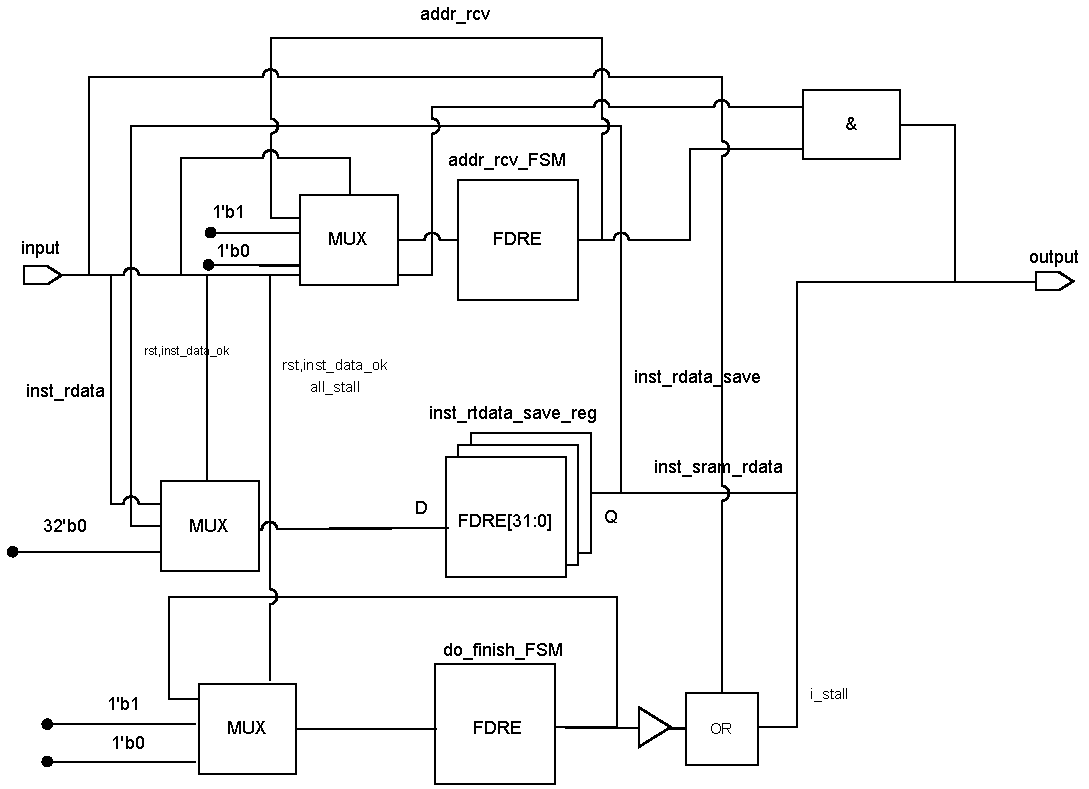
\includegraphics[width=0.9\textwidth]{image/isramtosramlike.pdf}
    \caption{sram转类sram接口通路图}
\end{figure}

\subsection{乘法器模块设计}
乘法器是我们小组自己设计的模块,其接口定义如下:
\begin{table}[H]
    \centering
    \begin{tabular}{ccccc}
        \hline
        信号名 & 方向 & 接口类型 & 位宽 & 说明 \\\hline
        clk & input & wire & 1 & 时钟 \\ 
        rst & input & wire & 1 & 复位信号 \\ 
        signed\_mul\_i & input & wire & 1 & 是否为有符号乘法 \\ 
        opdata1\_i & input & wire & 32 & 乘数1 \\ 
        opdata2\_i & input & wire & 32 & 乘数2 \\ 
        start\_i & input & wire & 1 & 开始信号 \\ 
        result\_o & output & reg & 64 & 结果 \\ 
        ready\_o & output & reg & 1 & 是否计算完成 \\ 
        mul\_stall & output & reg & 1 & 乘法全流水线stall \\ 

        \hline
    \end{tabular}
\end{table}

我们的乘法器分为三个状态,00表示空闲,01表示正在算第一拍,10表示算第二拍并且得到了结果,具体状态转移图如下:
\begin{figure}[H]
\centering
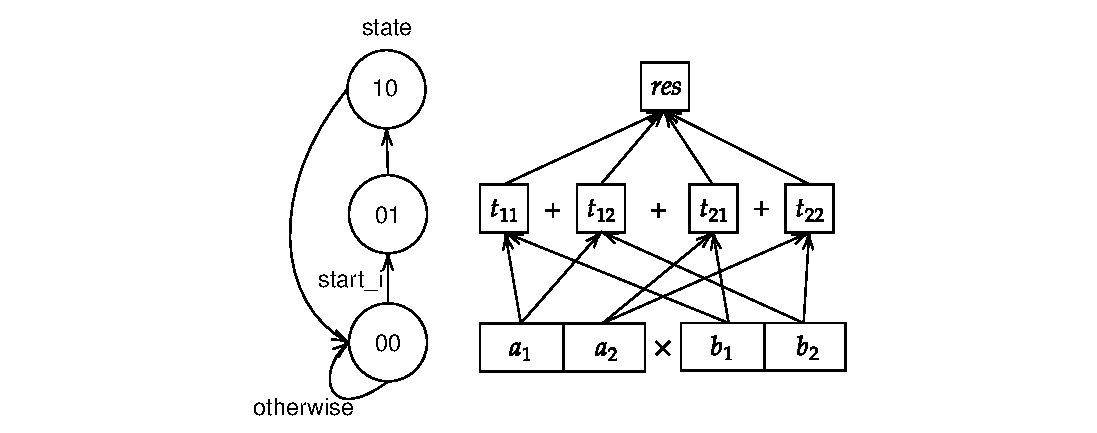
\includegraphics[width=\textwidth]{image/mul.pdf}
\caption{乘法器设计}
\end{figure}

乘法器的通路图如下:
\begin{figure}[H]
\centering
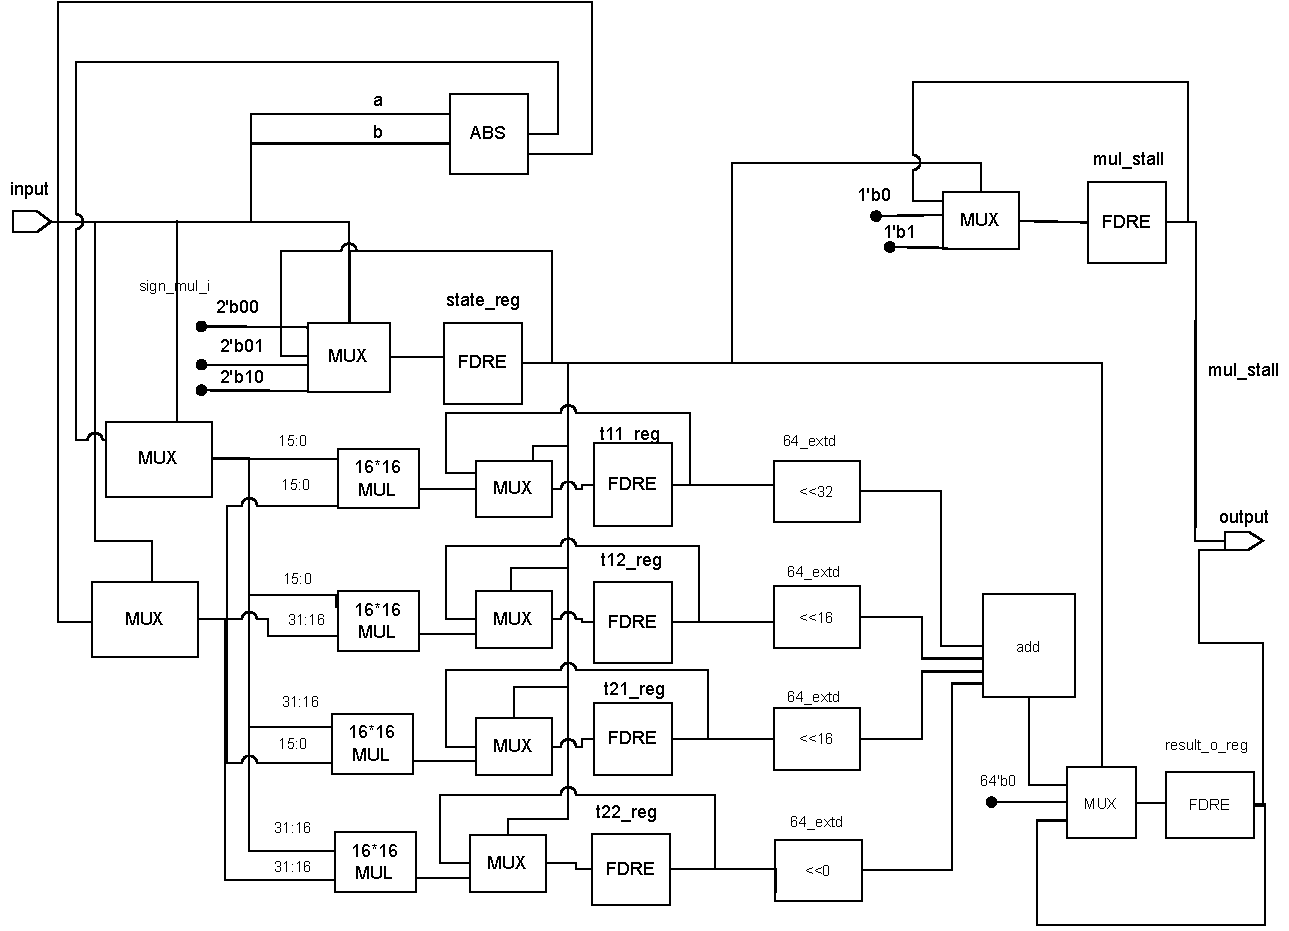
\includegraphics[width=0.9\textwidth]{image/mul2.pdf}
\caption{乘法器通路图}
\end{figure}